\section{Steady state spectroscopy}
\label{sec:SSS}

In the following, the steady state spectra for ZnTPP and ZnOEP in the two solvents toluene (Tol) and benzonitrile (BN) are analyzed.

First, we are comparing the spectra of the two different materials ZnTPP and ZnOEP as depicted in \cref{fig:ZnTPPZnOEP}.
\begin{figure}[h]
    \centering
    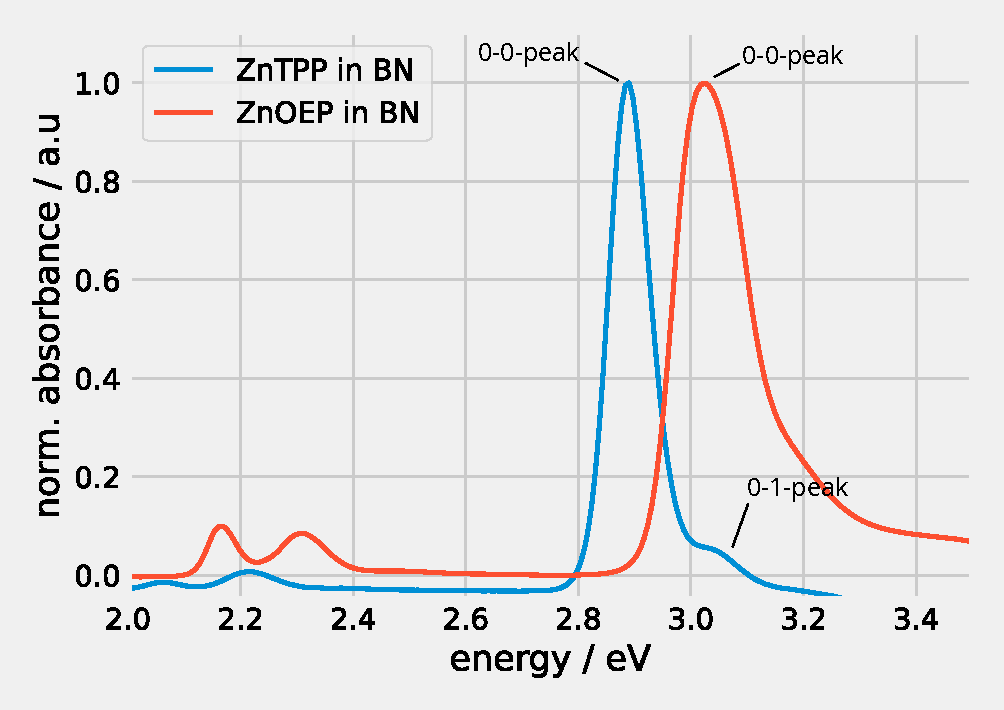
\includegraphics[width = 12cm]{Program/ZnTPPZnOEP.pdf}
    \caption{UV / VIS spectrum of ZnTPP and ZnOEP in benzonitrile.}
    \label{fig:ZnTPPZnOEP}
\end{figure}
The peak positions are analyzed using \textit{scipy.optimize.curve\_fit()}. The 0-0 transition of ZnTPP happens at 
\SI{2.89 \pm 0.01}{\eV} , whereas the same transition happens for ZnOEP \SI{3.03\pm 0.02}{\eV}. Furthermore, there are some peaks in the
range of of 2 to \SI{2.4}{\eV}. These peaks are stronger for ZnOEP
